\chapter{Visualisation}

\section{Visualisation Properties}
\index{Visualisation settings}

Some properties of the render window can be modified by selecting \cmd{Settings\ra} \cmd{Visualisation Settings...}. The dialogue that opens allows you to change several global properties of the render window.

For any rendered scene in computer graphics a light source\index{Light} has to be specified. This is basically the equivalent to the sun or a lamp in the room.
\begin{wrapfigure}{r}{0.4\textwidth}
   \vspace{-15px}
   \begin{center}
     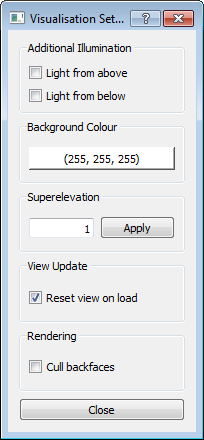
\includegraphics[width=0.36\textwidth]{dlg_vis_settings}
   \end{center}
   \vspace{-20px}
\end{wrapfigure}
The default setting in \ogs and many other tools is a light source identical with the camera, i.e. the light source always illuminates the part of an object in the render window that can be seen by the user. In some cases this illumination is not enough, though, and interesting parts of a rendered object may be covered by shadows. Therefore it is possible to switch on additional light sources above and below the object to ensure a full illumination of the scene.

The background colour\index{Background colour} of the render window can be changed to any arbitrary colour by clicking on the button displaying the current background colour. The button also displays the RGB-value of the currently selected colour.

A global superelevation\index{Superelevation} factor can be applied to all root objects in the visualisation pipeline. This overwrites all previously set superelevation factors and is especially useful when dealing with a large number of files, all of which should be assigned the same superelevation (e.g. when using \ogs projects, see section \ref{nativefileformats}).

Per default upon loading a new data set the 3D view is adapted to show the entire scene from above (i.e. the \emph{z+}-axis). This can be switched of by unchecking the ``Reset view on load'' option. This might be useful when making a series of screenshots with the exact same point of view.

Finally, it is possible to switch on backface culling\index{Backface culling}. This will result in rendering only triangles with normals directed towards the camera/observer. This improves rendering speed and may be useful for finding false ordered primitives.

\section{General Visualisation Options}
\label{genvisoptions}

For each graphics-object in the visualisation pipeline there a number of parameters that can be changed to make the object more easily distinguishable or to convey information contained in the data. These general options can be found in the \emph{Visualization Pipeline}-tab and are called ``Actor Properties'' (based on their use within VTK).

\begin{figure}[tb]
\begin{center}
\subfloat[Solid Color]{\includegraphics[width=0.3\linewidth]{colour-solid}\label{colour-solid}} \enspace
\subfloat[Default colour table]{\includegraphics[width=0.3\linewidth]{colour-default}\label{colour-default}}\enspace
\subfloat[User-defined colours]{\includegraphics[width=0.3\linewidth]{colour-user}\label{colour-user}}
\end{center}
\caption{Each object is assigned a random solid colour as well as a default colour table based on a temperature scale (from blue to red). The solid colour can be adjusted via the ``Diffuse Color''-option (see section \ref{genvisoptions}), the colour table can be adjusted by loading a user-defined *.xml file via the ``Add color table...''-option (see section \ref{specvisoptions}).} \label{fig:colours}
\end{figure}

Specifically these parameters are:

\begin{itemize}
\item \textbf{Diffuse Color:}\index{Changing Colour} Each item is assigned a colour which is used for rendering the object in 3D space. This colour can be changed here (see figure \ref{colour-solid}). If the item is assigned one or more scalar arrays (see next item) then this colour is displayed upon selecting \emph{Solid Color}.
\item \textbf{Active Scalar:}\index{Changing scalar values} Each visualisation object has an assigned colour called \emph{Solid Color} which is used in the rendering process (see above). However, some data sets contain additional information, such as individual values assigned to each point or mesh node as well as to any triangle or mesh element. Examples are material groups for meshes, the concentration of chemical substances, values assigned as boundary conditions, etc. Such information is called a \emph{Scalar Array} assigned to the data set and can be selected here. This additional data is then employed in the rendering of object (see figure \ref{colour-default}). In theory, an object can have any number of such scalar arrays. However, only one of these can be selected at any time.\\
    On the right side of the `Active Scalar'-pulldown-menu is also a button for re-adjusting the colour table. This might be necessary to use after parameter changes for certain filters, when the colour lookup table for this specific array is not automatically adjusted.
\item \textbf{Visible Edges:}\index{Edges} Some objects (such as meshes) are composed of a combination of lines (edges) and surfaces. While the colour of the surfaces can be set using the \emph{Diffuse Color}-button, the colour of the edges can be changed here. Furthermore the rendering of edges can be switched off entirely by unchecking the box next this option.
\item \textbf{Opacity:}\index{Opacity}\index{Transparency} This determines if an object appears to be completely or partially transparent or not. A value of $0$ (leftmost position of the slider) makes the object completely transparent, a value of $1$ (rightmost position) makes the object completely opaque.
\item \textbf{Scaling Factor:}\index{Scaling} Super-elevates the data by the given factor. Values $x>1$ will emphasise differences in height while values $0<x<1$ will compress the extent in $z$-direction.
\item \textbf{Translation:}\index{Translation} Any data set can be moved in x, y or z-dimension so data sets can be set in relation to each other for comparison or layered visualisation.
\end{itemize}


\section{Modification and Export Options}
\label{specvisoptions}

When right-clicking an object in the \emph{Visualisation Pipeline}, a number of options appear for modifying, converting or exporting that specific object. Not all options listed here apply to all types of pipeline items.

\begin{itemize}
\item \textbf{Add filter...:} Allows to apply a filter to the current object. There are many options and possibilities here and \ogs will add more filter-options over time. For details on that option see section \ref{filters}.
\item \textbf{Add color table...:}\index{Colour lookup tables} Allows the assignment of a specific colour table to the currently selected scalar array (see figure \ref{colour-user}). The colour table is loaded from a *.xml-file and has the same format as ParaView\footnote{ParaView is an open-source data analysis and visualisation application for VTK data. It can be downloaded at \url{http://www.paraview.org/}}-colour-lookup-tables.\index{ParaView}
    New lookup tables and can therefore be created or edited using ParaView and all colour tables used in \ogs can conversely be imported into ParaView.
    The option to change colour tables is available for all objects, although for image data it is not available via right-click but needs to be called as a filter (see section \ref{filters}).
\item \textbf{Convert to Mesh...:} Allows to convert an object of the VTK-data type ``Unstructured Grid'' to be converted into an \ogs mesh. Objects of that type are basically meshes that are stored in a different data structure than ``normal'' \ogs meshes. Therefore, this specifically allows the conversion of imported VTK-files to \ogs meshes. Upon conversion the converted mesh will also appear in the respective \emph{Data View.}\\
    This option is available for all objects of type ``VTK\_UN\-STRUCT\-URED\_GRID'' (i.e. all mesh objects).
\item \textbf{Convert Image to Mesh...:} Generates an \ogs mesh based on a given raster file (see figure \ref{Filter-Img4}). For more information, see section \ref{meshraster}. This options is only available for image data (i.e. raster files).
\item \textbf{Export to VTK:}\index{VTK export} All objects displayed the render window are technically VTK-objects. Choosing this option saves these objects in VTK-format to a file. They can then be used in any software supporting this format (e.g. Paraview).
\item \textbf{Export to OpenSG:}\index{OpenSG export} Converts objects into OpenSG format (*.osg). This is another open source graphics format. It is also the format used by the UFZ VisLab. Specifically, this also implies that \emph{anything} that can be visualised in \ogs can also be exported to OpenSG and be presented in the VisLab. This option only appears if an OpenSG-library is linked from \ogs.
\item \textbf{Export to FBX:}\index{FBX export}\index{Autodesk export}\index{Unity export} Converts objects into Autodesk format (*.fbx). This is yet another graphics format, originally used by AutoDesk but also supported by other graphics software such as Unity3D. This option only appears if an FBX-library is linked from \ogs.
\end{itemize}

\section{Applying Filters for Visualisation}
\label{filters}

In contrast to the options detailed in the previous section, filters are modifications of the actual graphics object to enhance, reduce or deform certain aspects of these objects.\footnote{One might argue that this definition also holds true for the assignment of specific color tables which is accessed via right-click on an object. This inconsistency originates in the data structures the objects are stored in and in defining an easy-to-use workflow for using this functionality.}.

Filters can be applied by right-clicking on an object in the visualisation pipeline and selecting \cmd{Add filter...}.\index{Adding filters}\index{Filter} A dialogue will open where a number of available filters can be selected. As with other visualisation functionality described before, filters will only be displayed for objects they can be applied to. However, this does not mean that the result of any filter will make sense for any object where it can be applied. Also note, that it is possible (and sometimes useful) to apply filters to filters to extract certain information bit by bit.
%
\begin{figure}[tb]
\begin{center}
\subfloat[Raster data]{\includegraphics[width=0.4\linewidth]{Filter-Img1}\label{Filter-Img1}}\enspace
\subfloat[Apply lookup table to image]{\includegraphics[width=0.4\linewidth]{Filter-Img2}\label{Filter-Img2}} \\
\subfloat[Image to bar chart]{\includegraphics[width=0.4\linewidth]{Filter-Img3}\label{Filter-Img3}}\enspace
\subfloat[Convert Image to Mesh]{\includegraphics[width=0.4\linewidth]{Filter-Img4}\label{Filter-Img4}}
\end{center}
\caption{\ogs functionality applicable to image-/raster-data.} \label{fig:filter:raster}
\end{figure}
%
A short description for all available filters is given in the following:

\subsubsection{Apply lookup table to image}
\bstart{Applicable to:} Image Data
\index{Colour lookup tables}

\bstart{Effect:} Applies a color table to images. The color table can be read from a *.xml-file. If no file is specified, a default color table is automatically generated, replacing grey values with a temperature scale (i.e. dark colours are blue, light colours are red). In the resulting image, certain gradients might be better discernable or certain values might be highlighted. See figure \ref{Filter-Img2}.

\bstart{Remarks:} \emph{This is similar to applying a pre-defined colour table to a geometry- or mesh object. The implementation as a filter for images is based on the very different structure of image objects in the graphics library VTK which is used for visualisation.}

\begin{figure}[tb]
\begin{center}
\subfloat[Geometry Data]{\includegraphics[width=0.4\linewidth]{Filter-Poly1}\label{Filter-Poly1}}\enspace
\subfloat[Points to Spheres]{\includegraphics[width=0.4\linewidth]{Filter-Poly2}\label{Filter-Poly2}} \\
\subfloat[Lines to tubes]{\includegraphics[width=0.4\linewidth]{Filter-Poly3}\label{Filter-Poly3}}\enspace
\subfloat[Extract cells by threshold]{\includegraphics[width=0.4\linewidth]{Filter-Poly4}\label{Filter-Poly4}}
\end{center}
\caption{\ogs functionality applicable to geometry data. In figure \ref{Filter-Poly2} ground water stations in the area have been emphasised. In figure \ref{Filter-Poly4} a threshold filter has been applied to the tube-filtered data from figure \ref{Filter-Poly3} to select only the river network of the depicted area from the geometric data.} \label{fig:filter:poly}
\end{figure}

\subsubsection{Apply texture to surface}
\index{Textures}\index{Raster files}\index{Raster files}\index{NetCDF files}
\bstart{Applicable to:} Surfaces, Meshes

\bstart{Effect:} Allows to map an image/raster on a surface or mesh. This might make sense for adding more information to a given object such as land use classes, precipitation, etc. Possible formats for loading textures include all supported raster formats as well as netCDF files (see \ref{Import File Formats}). An example is shown in figure \ref{Filter-Mesh4}.

\subsubsection{Elevation-based colouring}
\bstart{Applicable to:} Geometry, Meshes

\bstart{Effect: } Applies a colour to each point depending on the z-coordinate of that point, assuming that this denotes height in metres. The pre-defined colour scale starts with blue up to a height of $0$ metres (i.e. sea level), which is then slowly changing to green (150\,m) and yellow (450\,m) and then changing to red.. See figure \ref{Filter-Mesh2}.

\bstart{Remarks:} \emph{In theory these values can be changed. This is, however, currently not possible using the GUI. It is very easy in the source code, though, as this just constitues a predefined colour lookup table.}

\begin{figure}[tb]
\begin{center}
\subfloat[Multilayered Mesh]{\includegraphics[width=0.4\linewidth]{Filter-Mesh1}\label{Filter-Mesh1}}\enspace
\subfloat[Elevation-based colouring]{\includegraphics[width=0.4\linewidth]{Filter-Mesh2}\label{Filter-Mesh2}} \\
\subfloat[Extract cells by threshold]{\includegraphics[width=0.4\linewidth]{Filter-Mesh3}\label{Filter-Mesh3}}\enspace
\subfloat[Apply texture to surface]{\includegraphics[width=0.4\linewidth]{Filter-Mesh4}\label{Filter-Mesh4}}
\end{center}
\caption{\ogs functionality applicable to meshes.} \label{fig:filter:mesh}
\end{figure}

\subsubsection{Extract cells by threshold}
\index{Threshold filter}
\bstart{Applicable to:} Geometry, Observation Sites, Meshes

\bstart{Effect:} Geometric objects as well as mesh layers have unique IDs which allows to assign different colours to different objects. This filter furthermore allows to select a range of objects which should be displayed while all other objects are blanked out. This allows for the visualisation of one or more specified stratigraphic layer, polyline or mesh layer. See figures \ref{Filter-Poly4} and \ref{Filter-Mesh3}. The filter is always applied to the currently selected scalar array. For instance, given a mesh containing scalar arrays for material group and groundwater head, this filter may be used to select a range of materials (e.g. only materials with IDs 5--7) or regions with a certain groundwater head (e.g. $\text{head}>7.2\,m$).

\subsubsection{Generate contours based on scalar fields}
\index{Contour filter}
\bstart{Applicable to:} Meshes

\bstart{Effect:} Given a scalar field this filter will output contour lines of meshes containing 2D elements and contour surfaces for meshes containing 3D elements. The number of contours that should be displayed can be defined in the filter properties as well as the minimum and maximum value for the calculated contours. The chosen number of contours will that be calculated on the selected scalar field in equidistant intervals between the selected minimum and maximum value. The colours of the contours are automatically chosen based on these scalar values.

\subsubsection{Image to bar chart}
\bstart{Applicable to:} Image Data

\bstart{Effect:} Each pixel is assigned a bar depending on the grey value of the pixel. Also, the colour changes of that bar changes according to its height. See figure \ref{Filter-Img3}.

\bstart{Remarks:} \emph{This filter takes a lot of time for large images as the result becomes very complex from a computer graphics point of view. The intention is to use it for low resolution raster data of phenomena such as precipitation, etc.}

\emph{This is also a good example on the combination of the successive application of these filters. This one combines `Image to vertical lines', `Lines to tubes' and `Elevation-based colouring'.}

\subsubsection{Image to vertical lines}
\bstart{Applicable to:} Image Data

\bstart{Effect:} Plots vertical lines for every pixel of a raster with each line having a height depending on the raster's grey value.

\bstart{Remarks:} \emph{This is a filter that is needed for the correct application of other filters. It is probably not of much use by itself.}

\subsubsection{Lines to tubes}
\index{Tube filter}
\bstart{Applicable to:} Geometry, Observation sites

\bstart{Effect:} A geometric line has independent of the current zoom level always a thickness of $1$. This filter allows to assign a `real' thickness to line-objects that also changes according to the current zoom. See figure \ref{Filter-Poly3}.

\subsubsection{Points to spheres}
\index{Sphere filter}\index{Glyph Filter}
\bstart{Applicable to:} Geometry, Observation sites

\bstart{Effect:} A geometric point has independent of the current zoom level always a diameter of $1$. This filter allows to assign a `real' radius to point-objects that also changes according to the current zoom. See figure \ref{Filter-Poly2}.

\subsubsection{Surface filter}
\index{Surface filter}
\bstart{Applicable to:} Meshes

\bstart{Effect:} Extracts the outer surface of a mesh.

\bstart{Remarks:} \emph{This is a filter that is needed for the correct application of other filters. It is probably not of much use by itself.}
